\documentclass[12pt]{article}
\usepackage[spanish]{babel}
\usepackage[utf8x]{inputenc}
\usepackage[T1]{fontenc}
\usepackage{FiraSans}
\usepackage{amsmath}
\usepackage{graphicx}
\usepackage{float}

\renewcommand{\familydefault}{\sfdefault}

\begin{document}

\begin{titlepage}
\newcommand{\HRule}{\rule{\linewidth}{0.5mm}} 
\center


\includegraphics[scale=0.4]{images/logo-usm.png}\\
\vspace{0.6cm}
\textsc{\large INF480}\\[0.5cm] % Minor heading such as course title
\textsc{\Large Redes Complejas}\\[0.5cm] % Major heading such as course name

\HRule \\[0.4cm]
{ \huge \bfseries Tarea 1}\\[0.4cm] % Title of your document
\HRule \\[1.5cm]
 
\begin{minipage}{0.4\textwidth}
\begin{flushleft} \large
Florencia Ramírez\\
Sofía Riquelme
\end{flushleft}

\end{minipage}\\[2cm]

\vfill % Fill the rest of the page with whitespace

\end{titlepage}

\section{Introducción}
En este informe se presenta un análisis de la red 6 de la lista otorgada por el profesor. Esta red proviene de una red social "tipo Facebook" de estudiantes de la Universidad de California en Irvine; los pesos son cantidad de mensajes entre ellos.
\section{Datos básicos}
\subsection{Cantidad de nodos y aristas}
La red cuenta con 1899 nodos y 13.838 aristas

\subsection{Dibujo}
\begin{center}
    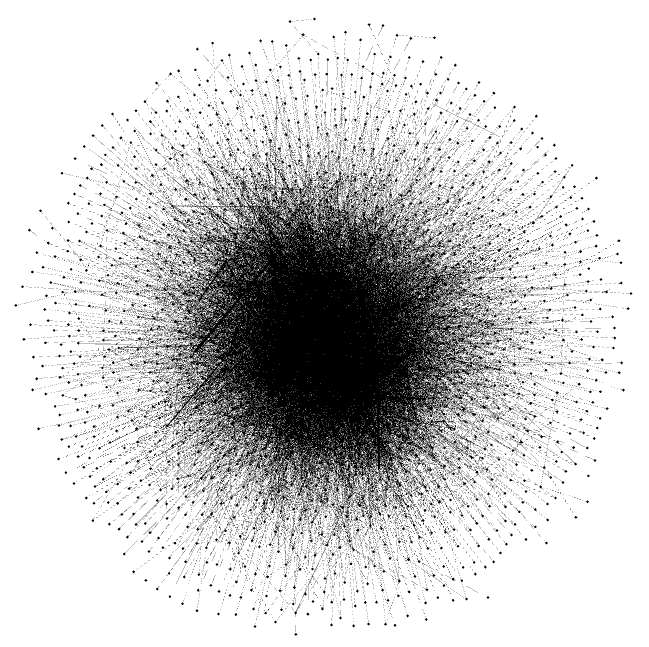
\includegraphics[scale=0.4]{images/dibujo_red.png}
\end{center}

\subsection{Conexidad}
La red es completamente conexa
\section{Análisis}

\subsection{Grados}

\begin{itemize}
    \item Grado mínimo: 1
    \item Grado máximo: 255
    \item Gráfico de distribución de grados: 
\end{itemize}
\begin{center}
    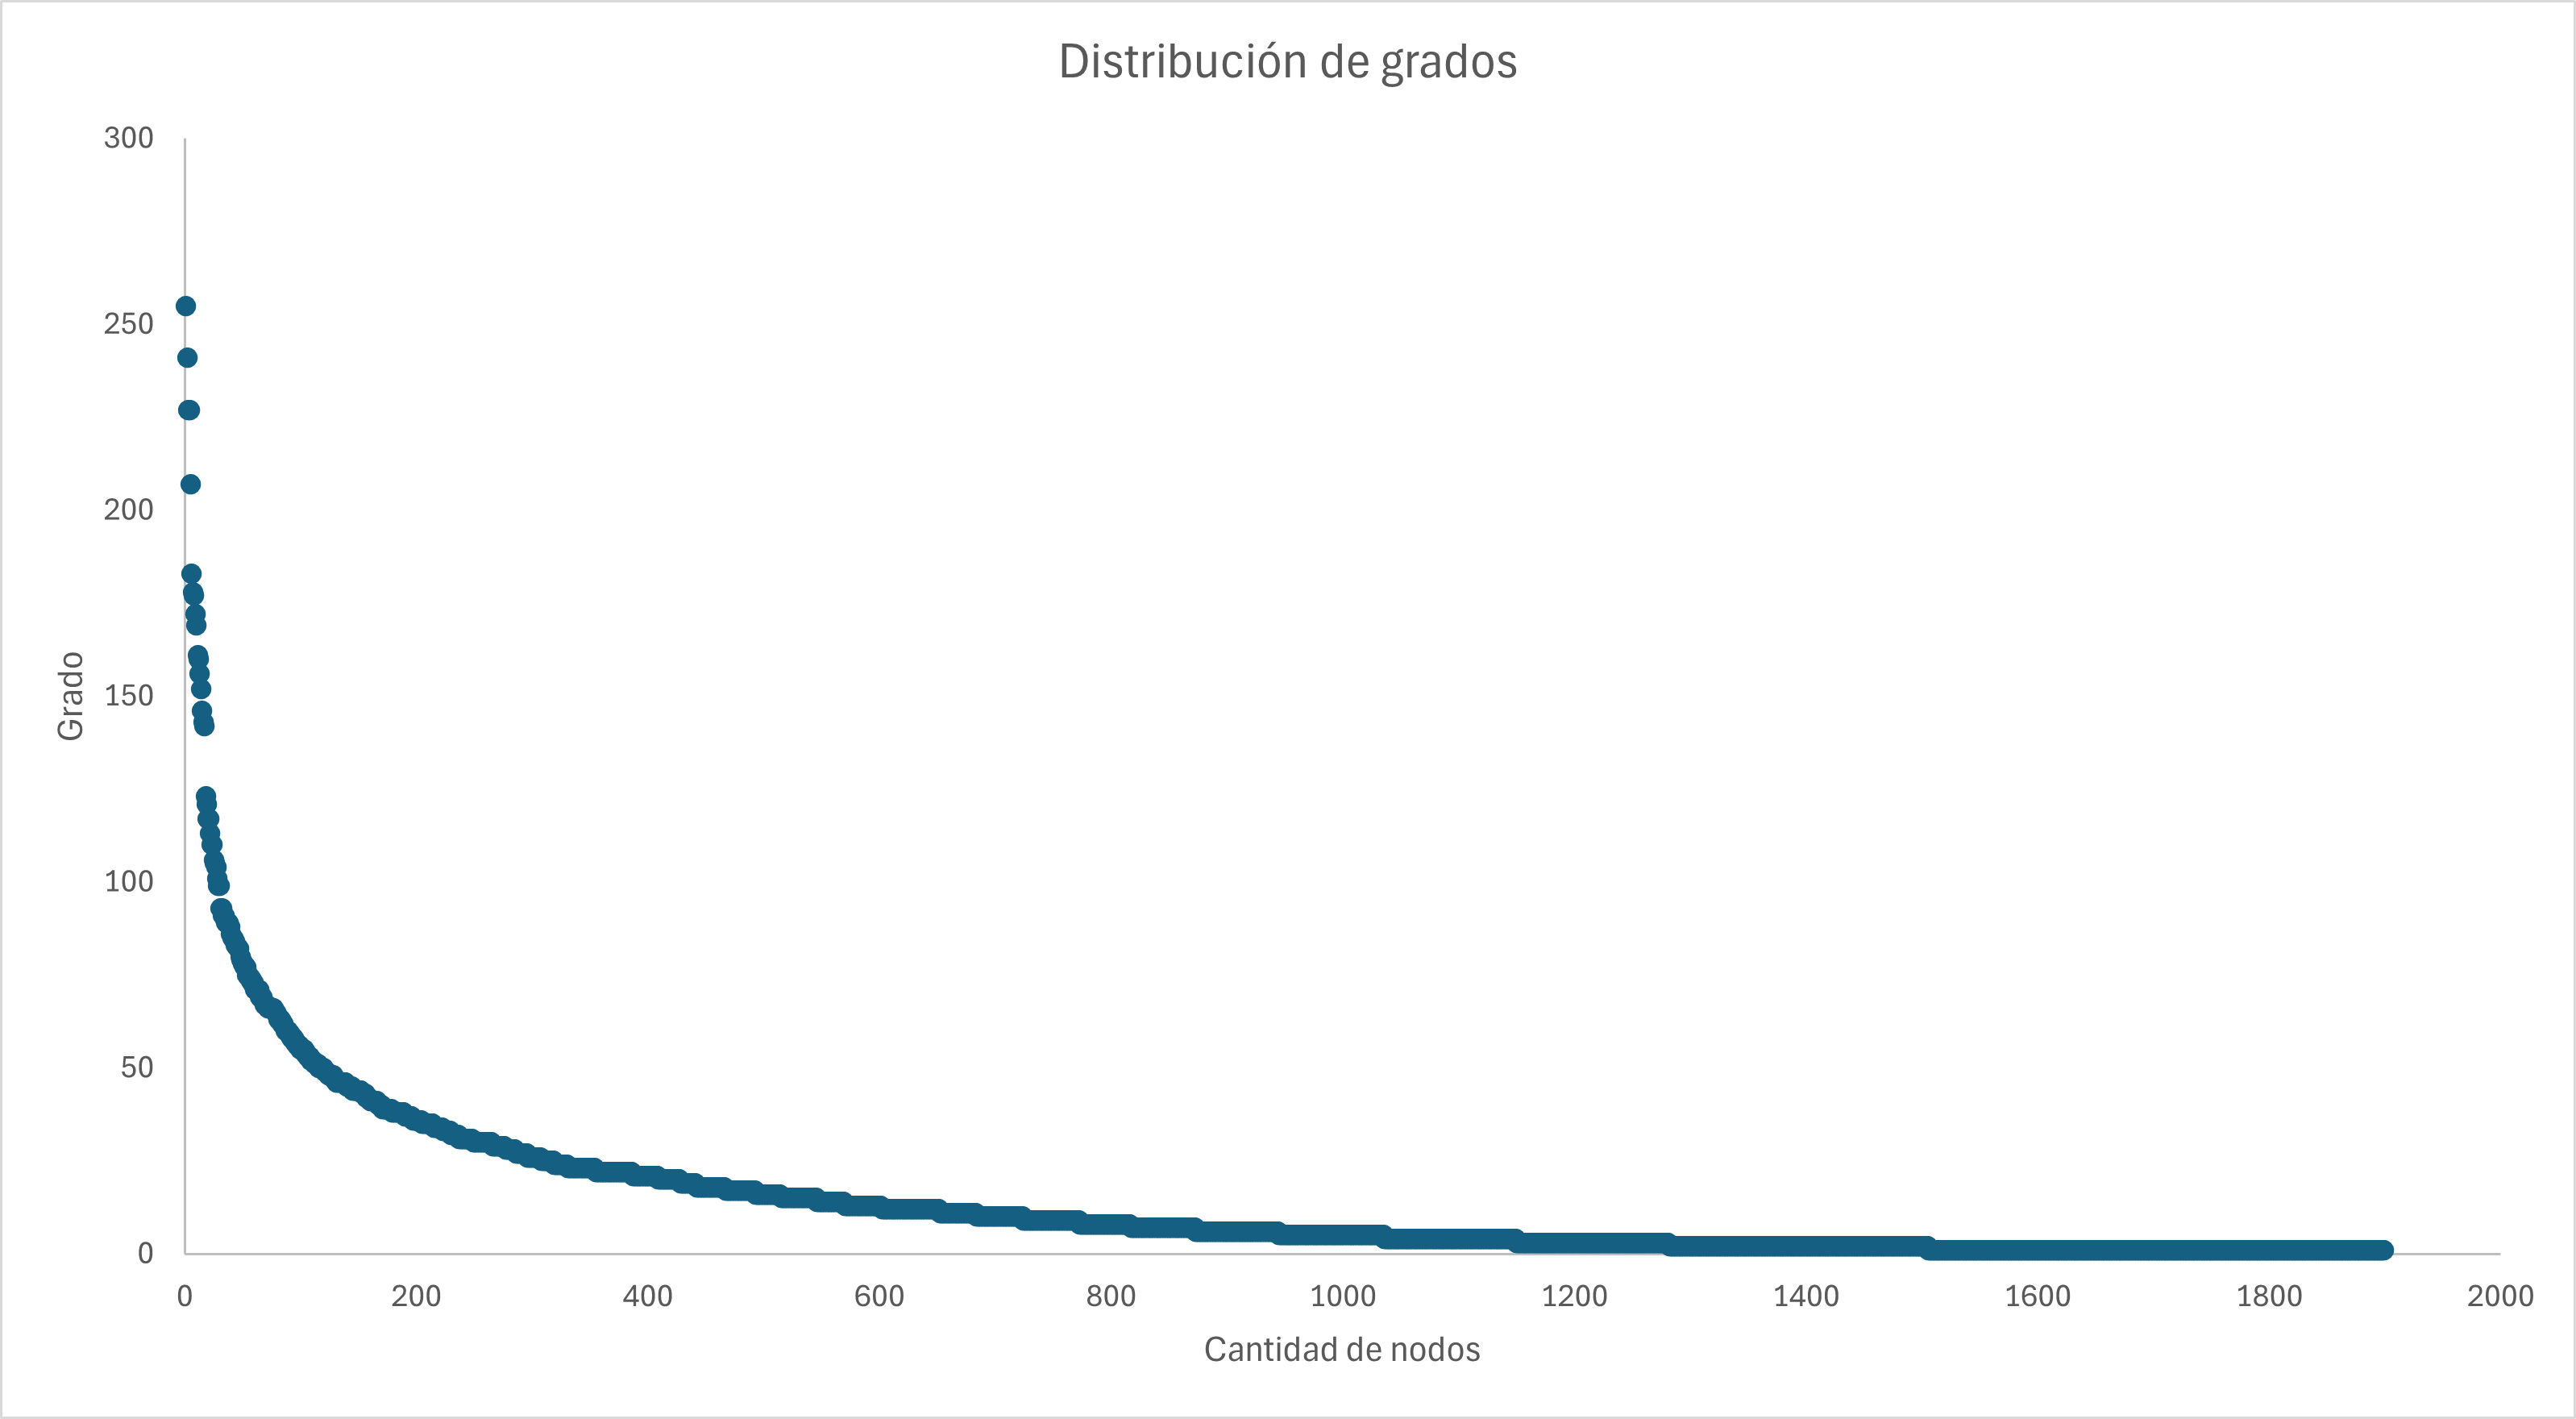
\includegraphics[scale=0.35]{images/distribucion_grados.png}
\end{center}
Con escala logarítmica:

\begin{center}
    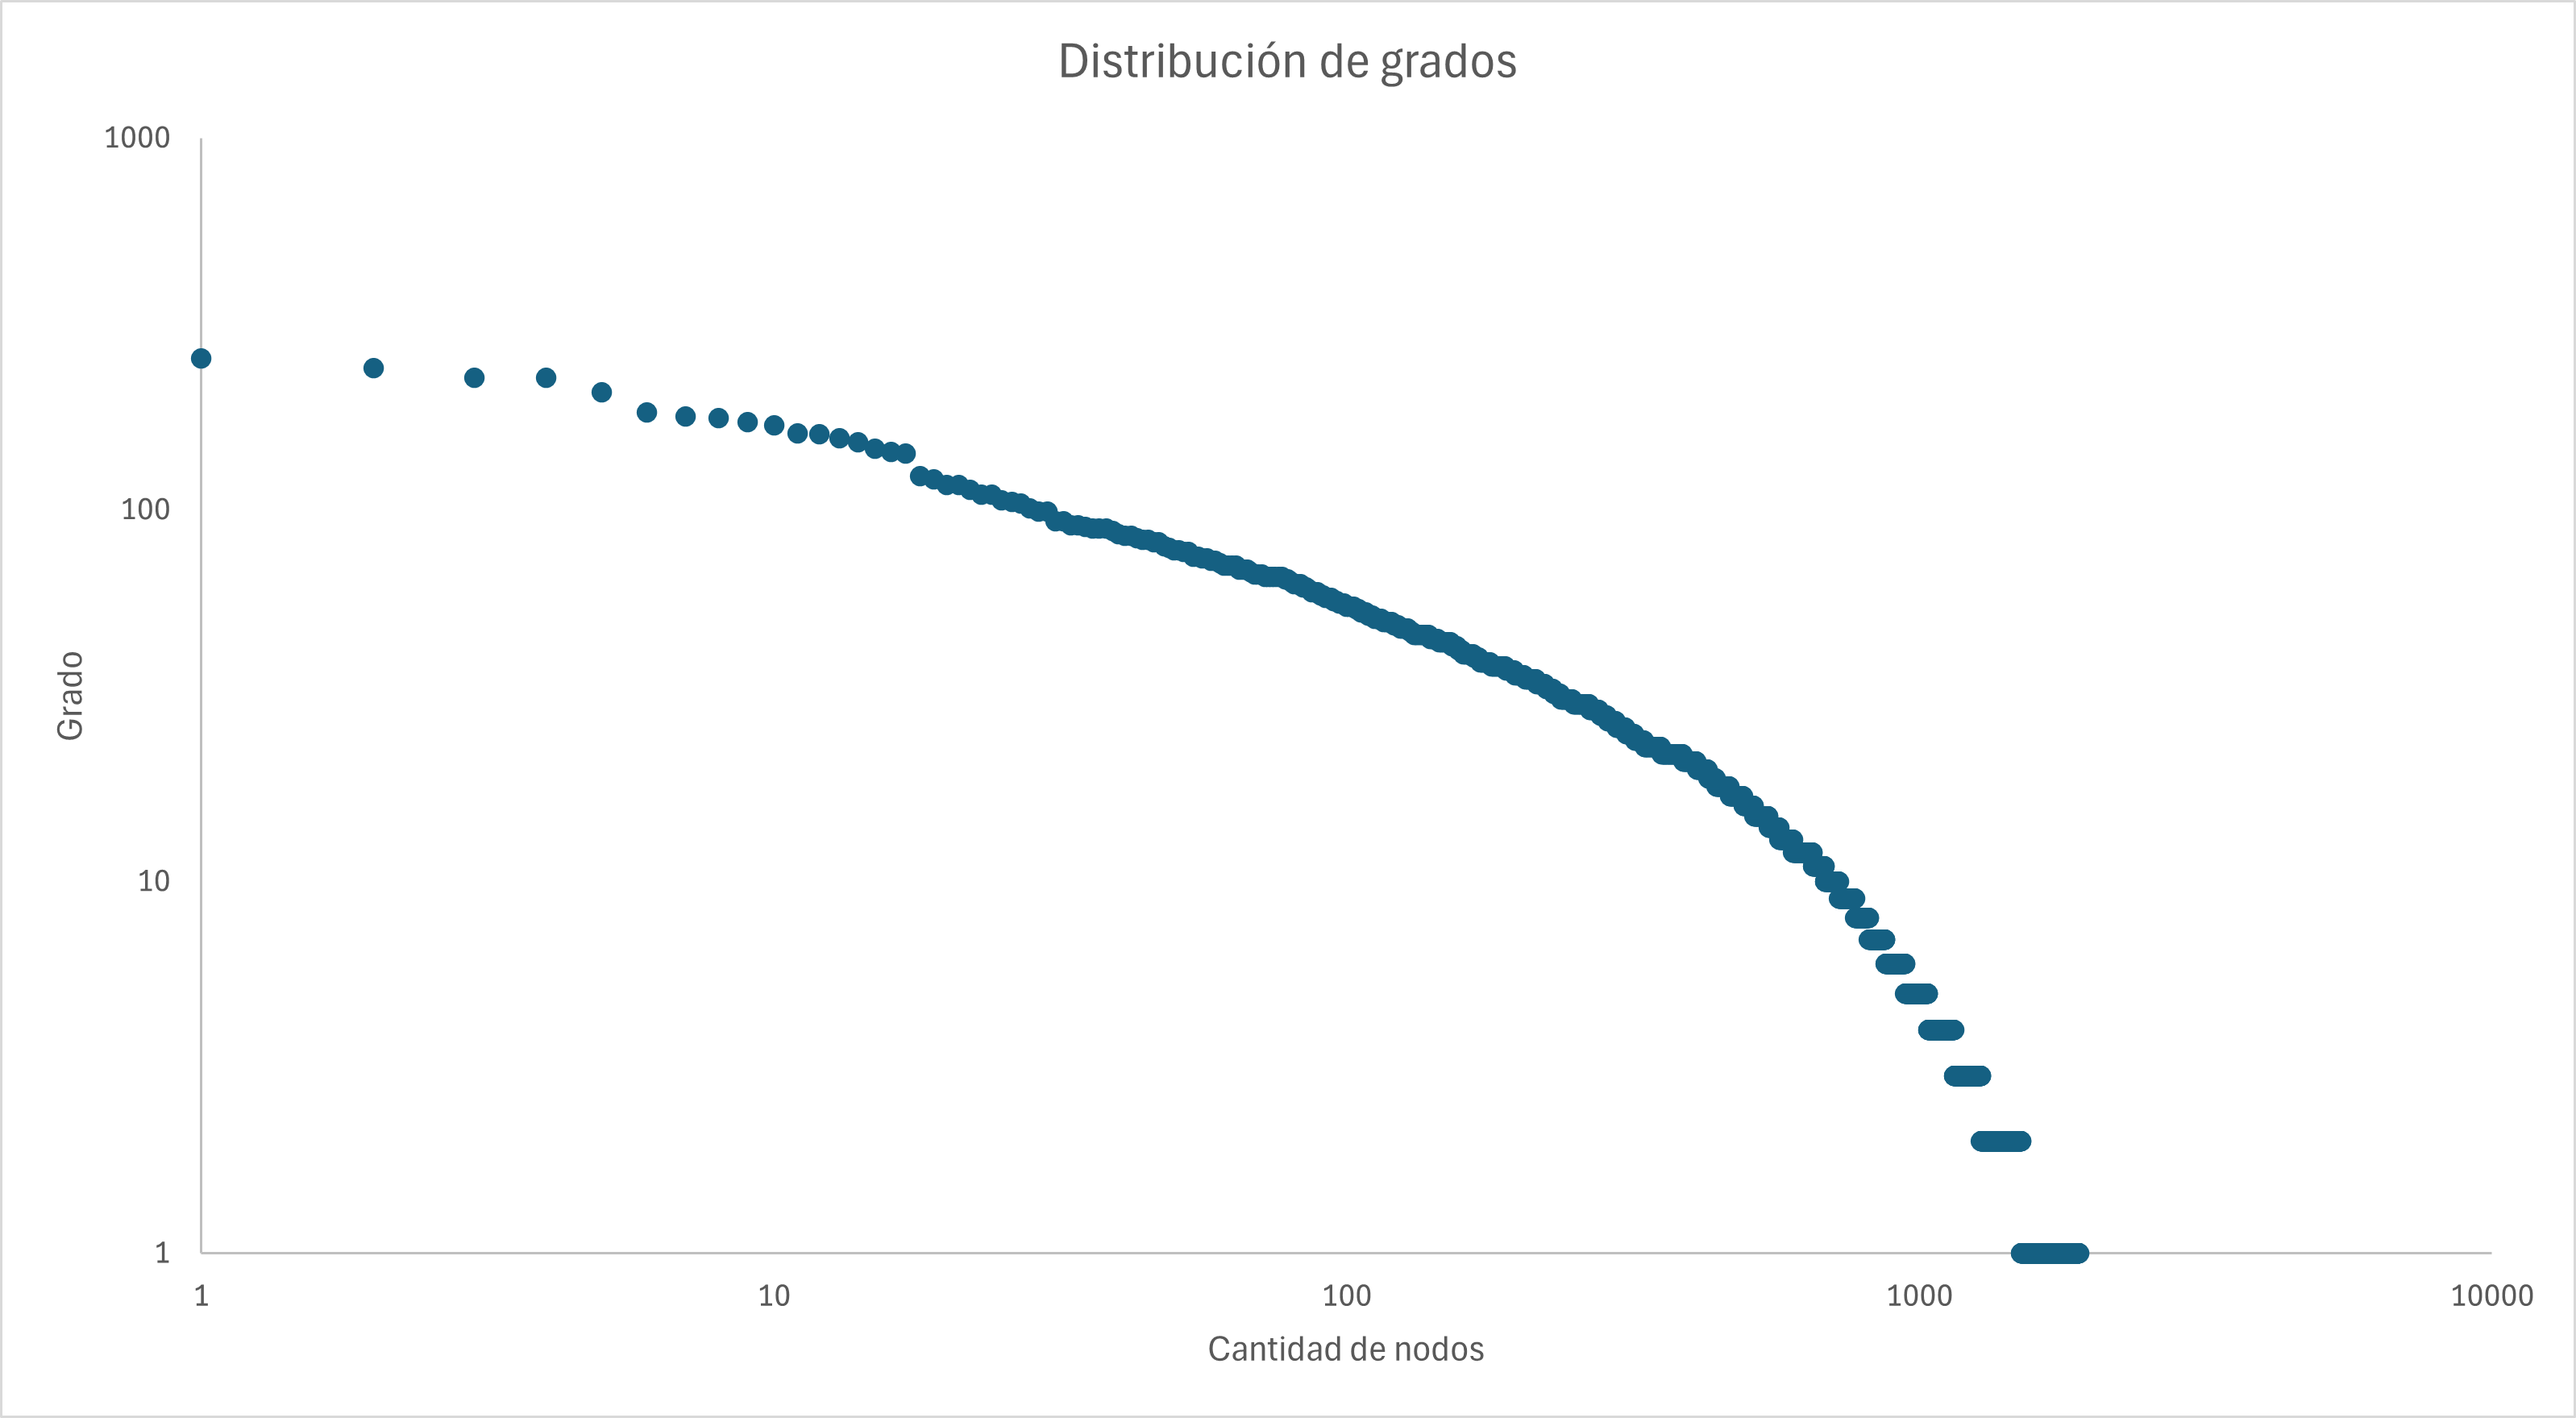
\includegraphics[scale=0.35]{images/distribucion_grados_log_log.png}
\end{center}

Se puede observar que si bien se esperaría que fuera una ley de potencia, no lo es 
\subsection{Distancias} 
La distancia promedio entre los nodos es de 3.055 y el diámetro de la red es 8
(hay que ver si es que se justifica)

Determine la distancia promedio entre los nodos, y el diámetro de la red. ¿Se justifica hablar de efecto small world?

\subsection{Transitividad} 
Determine el coeficiente de clustering local de la red. ¿Hay transitividad alta?

\subsection{Centralidad}  
Determine la centralidad de intermediación, PageRank y cercanía de cada nodo. Expórtelas a alguna herramienta de análisis y explore qué tan relacionadas están entre sí, y con el grado del nodo (en particular, haga gráficos de dispersión de grado y PageRank, PageRank e intermediación, etc.). Identifique las mayores desviaciones (nodos con centralidad alta según una métrica y baja según otra) e intente explicarlas en función de la estructura de la red. Obtenga imágenes de la red coloreada según los valores de las distintas centralidades. [Nota: Gephi es un poco críptico. Para calcular intermediación o cercanía hay que decirle que calcule "diámetro de la red", que no tiene nada que ver.]

\subsection{Núcleo/Periferia}
Determine la profundidad de k-cores (el máximo k para el cual el k-core es no vacío), y la cantidad de nodos en cada k-shell (cada “capa de la cebolla” en k-cores).

\subsection{Comunidades} Aplique el algoritmo de Lovaina de detección de comunidades (Gephi lo trae por defecto). Si usa parámetros distintos al default, especifique. Reporte la cantidad y el tamaño de las comunidades encontradas, y el valor de modularidad conseguido. Use las comunidades obtenidas para colorear la red. ¿Se aprecia en el gráfico la estructura de comunidades? ¿Interactúan todas con todas, o cada comunidad se relaciona con unas pocas de las demás? [Aquí si hace falta puede jugar un poco más con las opciones de layout, para buscar un buen dibujo de la red.]

\subsection{Asortatividad}
Calcule el coeficiente de correlación de Newman para medir la asortatividad de la red. ¿Le parece asortativa, disasortativa, o ninguna?

\subsection{Modelo estructural} Genere 10 redes aleatorizadas que compartan la distribución de grados de su red, y para cada una de ellas determine la modularidad (aplicando el mismo algoritmo de Lovaina), el coeficiente de correlación, el coeficiente de clustering local, y la profundidad de k-cores. Compare los valores con el obtenido para su red: ¿pueden explicarse sus valores a partir de la distribución de grados, o parecen ser propiedades específicas de la red?


\end{document}